\chapter{Optimization}
\label{optimization}
The previous chapter introduced the means to enable parallel execution of code via tasks and establish communication between tasks via shared resources. In order to make the communication thread-safe, synchronization statements were presented which provide synchronization contexts of atomic thread-safe blocks for the shared resources that they synchronize. For the purpose of both simplicity of the design and thread-safety of the user-code, conservative restrictions were made: in the variability of the code and the scopes of synchronization contexts. While this strategy simplifies the construction of correct programs for the user, it may induce unnecessary serialization during program execution if potential data hazards will actually never manifest at runtime \cite{SpeculativeLockElision}. While the synchronization overhead reflects the optimization potential in the time-wise dimension, there is also a space-dimension which originates from the way mutexes are used in the implementation. 

\section{Space Optimization}
As was briefly addressed in \ref{sharedTypesTranslation}, the runtime memory consumption of the translated code is extended by the amount of memory that is occupied by the mutex maintenance. In addition to the obvious memory consumption of the handle and some internal management data, the realization of the choice to make mutexes robust against recursive locks requires a counter field to be maintained throughout the lifetime of each mutex. This property impairs both the space and computation time overhead of the implementation unnecessarily if shared resources are never recursively synchronized. If such cases are detected (which they are, as will be shown in the next section), the generator could decide to declare the according mutexes as non-recursive. This optimization is left for future extensions of ParallelMbeddr. Another starting point for the optimization of space consumption would be the reduction of padding, i.e. unused data, that is automatically introduced by the compiler into the struct instances of shared resources. Padding is added into structs in order to retrieve data from memory more efficiently by aligning it along proper addresses \cite[p.~27]{MemoryAsAProgrammingConcept}. The amount of padding that is inserted depends on the difference among the byte sizes of the individual fields, as well as the order of these fields \cite{MemoryAsAProgrammingConcept}. Since the ``art of C structure packing''\footnote{See http://www.catb.org/esr/structure-packing/, accessed: 2014-08-19, for details.} is no trivial task and space optimization is no primary concern of this paper, according work is left to future research.



\section{Time Optimization}
Various optimizations for lock-based synchronizations have been conceived. The general goal of all approaches is to minimize the overhead of synchronization measures. Among others, this can be accomplished in two different ways: First, the amount of synchronization management, i.e. the time spent for acquiring and releasing locks, can be reduced by diminishing the number of performed locks. This technique is called \textit{lock elision}. Secondly, the waiting time of threads for the release of locks which they try to acquire, also known as \textit{lock contention}, can be diminished. While the classic approaches try to optimize the code at compile-time, increasing effort is performed towards optimizations which occur at run-time. The latter kind primarily resides in the domain of the transactional memory model \cite{SpeculativeLockElision}\cite{ARuntimeSystem}. Due to the complexity and overhead of such techniques this thesis focuses on compile-time optimizations.

The applicable measures for optimizations differ in their coverage of `perceived potential' and their performance. Superior techniques often require more comprehensive information, which, in turn, demands more sophisticated analyses. Such analyses, however, usually come with an increase of complexity. Typical candidates are \textit{pointer analysis} and \textit{data-flow analysis}.

\subsection{Pointer Analysis}
Pointer analysis, also known as \textit{points-to analysis}, tries to find the set of memory locations to which a pointer may point \cite{PointerAnalysisForStructuredParallelPrograms}. Pointers with coinciding pointed-to addresses are called \textit{aliases} of one another (in the following, though, `alias' will rather be used as the pointed-to destination which, for shared resources, remains its value and can, thus, be identified with the stored shared resource). The information delivered by the pointer-analysis will be heavily used in the static analysis of this chapter. The following example illustrates the basic principle of pointer analyses. At the end of the if-else statement, \CODE{p} may point to the location of either \CODE{v} or of \CODE{w}. Due to the copy-semantics of assignments in C, \CODE{q} will have the same value as \CODE{p} after the assignment in line 5. \CODE{p} can therefore be regarded as an \textit{alias} of \CODE{q}.
\begin{ccode}{caption=Aliases of a pointer}
int32 v, w;
int32* p;
if (condition)  p = &v;
else            p = &w; 
int32* q = p;
\end{ccode}
The quality of a pointer analysis is reflected by its precision. Two properties -- that are relevant for this work -- influence the precision: whether the analysis is \textit{flow-sensitive} or \textit{-insensitive} and whether it is \textit{inter-procedural} or \textit{intra-procedural} \cite{ProgramAnalysisAndSpecialization}.\footnote{The latter property is also called context-sensitivity \cite{CloningBasedContextSensitive}.} The first property distinguishes whether the particular flow of data and with it the order of statements is taken into account of the analysis. For an illustration, the previous code listing is reconsidered. In a flow-insensitive analysis, the set of locations for \CODE{p} would contain the locations of both \CODE{v} and \CODE{w} in either branch. A flow-sensitive analysis, on the other hand, would precisely assign \CODE{v} or \CODE{w} to the points-to set (differing from above definition of aliases, in the following also called \textit{alias set}) of \CODE{p}. The second property distinguishes how precisely the calculation of points-to sets regards effects across functions, i.e. the context flow across function calls. The following example shall illustrate the difference between the two shapes. According to Andersen, an intra-procedural analysis would merge the calls of \CODE{bar()} so that the points-to set of \CODE{p} would contain both \CODE{v} and \CODE{w}. Likewise, the sets of \CODE{vP} and \CODE{wP} would contain the same elements. On the other hand, an inter-procedural analysis would distinguish the calls so that, in the end, the sets of \CODE{vP} and \CODE{wP} would contain exactly \CODE{v}, respectively \CODE{w}.
\begin{ccode}{caption=Aliases across function calls}
void foo() {
  int32 v, w;
  int32* vP = bar(&v);
  int32* wP = bar(&w);
}
void bar(int32* p) {
  return p;
}
\end{ccode}
At times, it is necessary to not compute the aliases that a pointer can have in the course of a program run. Instead the set of locations that a pointer will point to on every possible path through the program might be needed.\footnote{An application of this demand will be shown later on.} While the former is called a \textit{may point-to} analysis, the latter is called a \textit{must point-to} analysis \cite{ProgramAnalysisAndSpecialization}.
Currently, mbeddr does not provide any form of pointer analysis.

\subsection{Optimization Opportunities}
Static analysis offers a variety of optimization opportunities. These differ both in their optimization potential and the information needed for their realizations. Due to the similarity of shared resources to the synchronization concept of Java's monitors and the ongoing research in this area, the optimization ideas were (mainly) influenced by the according literature \cite{StaticAnalysesForJava}\cite{JavaTheoryAndPractice}\cite{DoJava6Threading}. The opportunities are arranged in the order in which they are applied in ParallelMbeddr. The first three of the following paragraphs concern themselves with the \textit{elision} of unnecessary locks and, hence, the computational overhead of synchronization management. The fourth focuses on the reduction of lock contention.

\subsubsection{Single-Task Locks}
The most obvious case in which locks for shared resources can be removed is when synchronized data is only accessed by one task. This may happen for a limited amount of time, for instance in the time span from the declaration of a local variable of a shared resource to its first sharing with other tasks:
\begin{ccode}{caption=Shared resource with a `temporary' single-task lock}
void foo() {
  shared<int32> v;
  shared<int32>* vP = &v;
  init(vP);
  |task(vP)|;
}

void init(shared<int32>* var) {
  sync(var as varToSet) {
    varToSet->set(0);
  }
}

void task(shared<int32>* var) {
  sync(var as varToGet) {
    int32 val = varToGet->get;
  }
}
\end{ccode}
Whereas \CODE{varToSet} in \CODE{init()} does not need to be synchronized, since it is not yet shared with another task, \CODE{varToGet} obviously needs to be synchronized inside \CODE{task()}.

Furthermore, during the whole run of a program, a shared resource could be accessed by one task only. This can happen if the programmer does not work attentively. More importantly, the re-use of existing data structures and according functions for single-task data can cause the same effect. For instance, a thread-safe queue and functions to manage this queue could be re-used by the user for data that resides in only one task. It would then be helpful to distinguish the necessity of locks (i.e. sync resources) depending on the use of queue.

\subsubsection{Read-only Locks}
In ParallelMbeddr, shared resources might actually never be set. For primitive data, e.g. of the type \CODE{shared<int32>} this should seldom be the case, if the user creates the code carefully. However, he might decide to use structs in order to pack independently synchronizable data:
\begin{ccode}{caption=Shared resource with read-only lock}
struct QueueContainer {
  shared<Queue>   queue;     // Queue is given as a black-box
  shared<boolean> isFull;
  shared<int32>   itemCount;
}

void foo() {
  shared<QueueContainer> queueC;
  shared<QueueContainer>* queueCP = &queueC;
  // ...
  sync(queueC) {
    sync(&queueC.get.isFull as isFull) { isFull->set(true); }
  }
}
\end{ccode}
Because of the semantics for variables of shared resources, \CODE{QueueContainer} can never be overwritten by another value. This is accomplished by mbeddr's non-typesystem rules. Therefore, any synchronization of \CODE{queueC} and any of its aliases is not necessary. However, the user still needs to pack the data into a shared resource in order to be able to safely share it with other tasks. Although the IDE could infer that \CODE{queueC} never needs to be synchronized, the user has to annotate the synchronization in line 11. If, on the other hand, such synchronization would not be required for \CODE{queueC}, additional synchronizations would have to be added if \CODE{QueueContainer} is eventually equipped with non-shared data. The current approach omits this change.\footnote{Of course, it is discussable which approach would be better.} Nevertheless, the compiler should take care of eliminating locks for such data. If functions are called with both read-only shared resources and written shared resources as argument data, the necessity of synchronizing them might depend on the respective calls (equivalent to single-task locks). This could for instance be the case for logging functions which only read the data of their arguments that shall be logged.

\subsubsection{Recursive Locks}
ParallelMbeddr does not prevent the user from acquiring locks for shared resources recursively. Instead, due to the scoping rules of synchronization resources and their contexts the programmer might be forced to synchronize shared resources recursively. In chapter \ref{mapReduceApproach}, such a case arises for the access to a thread-safe queue implementation.

\subsubsection{Lock Contention}
Besides the removal of locks, an important optimization opportunity is the reduction of lock contention. In order to accomplish this goal, the synchronization lists of synchronization statements should be shrunk to the absolute minimum. In the following, this technique is called \textit{lock narrowing}. For instance, the user might decide to apply coarse-grained synchronization by defining one big synchronization context inside a function:

\begin{ccode}{caption=Lock contention caused by coarse-grained synchronization}
void calculate(shared<double>* result) {
  sync(result as myResult) {
    double pi = calculatePi(); // do something that is expensive and unrelated to the argument
    myResult->set(pi);         // now use myArg
    log(pi);                   // again, something unrelated
  }
}

double calculatePi() {...}
void log(double arg) {...}
\end{ccode}

The statements in lines 3 and 5 do not make any use of the synchronized argument \CODE{result}. Hence, it would be safe to move these statements out of the synchronization context:

\begin{ccode}{caption=Optimization of lock contention}
void calculate(shared<double>* result) {
  double pi = calculatePi();
  sync(result as myResult) { myResult->set(pi); }
  log(pi);
}
\end{ccode}

One could argue that synchronization lists could even be split into multiple parts in order to separate statements whose evaluations access the current synchronization resources from those that do not:

\vspace{4mm}
\begin{minipage}{1\textwidth}
\begin{minipage}{0.37\textwidth}
\begin{ccode}{}
void increment(shared<int32>* c) {
  int32 current, next;
  sync(c as myC) {
    current = myC->get;
    next = current + 1;
    myC->set(next);
  }
}
\end{ccode}
\end{minipage}
\begin{minipage}{0.2\textwidth}
\begin{center}
$\longrightarrow$

split
\end{center}
\end{minipage}
\begin{minipage}{0.42\textwidth}
\begin{ccode}{}
void increment(shared<int32>* c) {
  int32 current, next;
  sync(c as myC) { current = myC->get; }
  
  next = current + 1;

  sync(c as myC) { myC->set(next); }
}
\end{ccode}
\end{minipage}
\captionof{lstlisting}{Aggressive narrowing introduces possible data-race}
\end{minipage}
\vspace{2mm}

Yet, with such an aggressive strategy, the optimizer might split the code across data dependencies which were formerly taken account of in the code by the scope of a synchronization statement. For instance, in the previous example, the split does not take into consideration the data dependencies between \CODE{current}, \CODE{next} and \CODE{myC}. Therefore, when another call of \CODE{increment()} is executed in an interleaved fashion, the resulting code introduces data races for the shared resource that \CODE{c} points to.

\subsection{Performed Optimizations}
The optimizations that were performed in this work are direct realizations of the aforementioned optimization opportunities. For the lack of supporting analyses in mbeddr at the time that this thesis was written, the optimizations assume that all threads are executed simultaneously in order to fit the scope of this work. Thus, since mbeddr was missing a pointer-analysis, at first a simplified pointer analysis for the application in the optimization algorithms was conceived. In this analysis, differing from the usual approach, a separate alias set is computed for each local variable, argument and reference of both kinds.\footnote{The analysis is therefore \textit{inclusion-based}, i.e. alias sets may overlap \cite{CloningBasedContextSensitive}.} Additionally, divergent from the usual terminology, an alias in this context is a variable or argument of type \CODE{shared<t>}. These differences result from the following facts

\vspace{10mm}
\begin{itemize}
\item only shared resources are considered;
\item shared resources are bound to memory locations, as they may not be rewritten;
\item shared resources inside structured data like arrays and structs are not considered.
\end{itemize}

Also, it is assumed that everything which has a type \CODE{shared<t>} or \CODE{shared<t>*} (i.e. variables, arguments and expressions) has an alias set. For the former type, this is clearly the location of the resource itself.

\subsubsection*{Pointer analysis}
As was mentioned before, the analysis that was implemented in the course of this thesis makes several simplifications in order to fit the scope of this work. The analysis is intra-procedural. For the lack of assignment consideration flow-sensitivity is irrelevant for the regarded language concepts. The analysis can either compute \textit{must point-to} or \textit{may point-to} alias sets.
As a starting point, a simplified directed data-flow graph is constructed. The nodes of this graph consist of local variable declarations, arguments\footnote{Although generally, arguments are the values that are passed to function parameters, in the course of this work, no such distinction is made. Instead, the formal function parameters are called arguments and the values, which are passed to functions, are called argument values. This terminology is closer to the one established in mbeddr.} and references to either kind. For each reference $r$ to a local variable or an argument $x$, an arc $(x, r)$ is added to the graph. Furthermore, for each local variable $v$ of type \CODE{shared<u>} or \CODE{shared<u>*}, whose initialization expression is a reference $r'$ to a local variable or argument of the same type, an arc $(r', v)$ is added. The same is done for local variables of type \CODE{shared<u>*} whose initialization expressions reference local variables or arguments of type \CODE{shared<u>} by address. Equivalently to local variables and initialization expressions, arcs $(r, a)$ are added to the graph for according pairs of argument values $r$ and arguments $a$.

Figure \ref{fig:dataFlowGraph} illustrates the principle: For each reference to the local variable \CODE{container}, an edge going from \CODE{container} to this reference is inserted. The same happens for the function arguments \CODE{c} and \CODE{cV}, as well as for the local variables \CODE{myC} and \CODE{myCV}. Furthermore, an edge connects the \CODE{container} reference with the argument \CODE{c}. On the other hand, \CODE{cV} has no incoming edge, since due to the simplifications of the algorithm only such expressions may be nodes that are direct or address (\CODE{\&}) references to variables or arguments:

\begin{minipage}{1\textwidth}
\begin{center}
\begin{minipage}{0.4\textwidth}
\begin{ccode}{}
int32 main(int32 argc string[] argv) {
  shared<shared<int32>> container;
  sync(container) { 
    foo(&container, container->get); 
  }
}

void foo(shared<shared<int32>>* c, 
         shared<int32>* cV) {
  sync(c as myC, cV as myCV) {
    cV = myC->get;
    myCV->set(0);
  }
}
\end{ccode}
\centering $\Downarrow$ resolve named resources $\Downarrow$ 
\begin{ccode}{}
...
void foo(shared<shared<int32>>* c, 
         shared<int32>* cV) {
  shared<shared<int32>>* myC = c;
  shared<int32>* myCV = cV;
  sync(myC, myCV) {
    cV = myC->get;
    myCV->set(0);
  }
}
\end{ccode}
\end{minipage}
\begin{minipage}{0.58\textwidth}
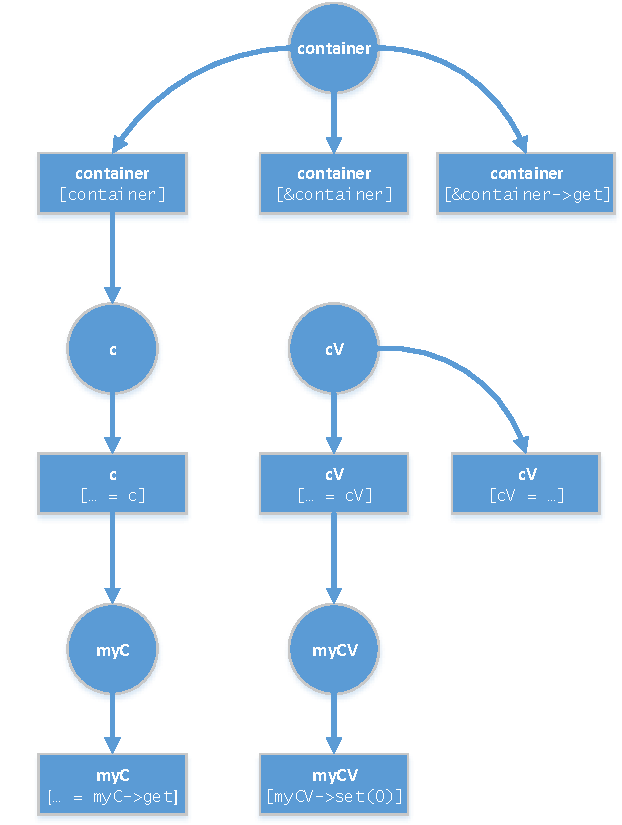
\includegraphics[scale=0.98]{pics/DataFlowDiagram}
\end{minipage}
\end{center}
\captionof{figure}{Simplified data-flow graph of shared resources}
\label{fig:dataFlowGraph}
\end{minipage}

The data-flow graph is used to perform a pointer analysis. The output of the analysis is a directed alias graph whose nodes comprise the nodes of the data-flow graph. Each arc $(u, v)$ of the alias graph connects a variable, argument or reference $u$ with a variable or argument $v$. In doing so, either $v$ is an alias for $u$ or $u$ refers to another variable which has an arc to $v$.\footnote{This may for instance be the case for a local variable of a shared resource pointer which is initialized with the value of another such pointer which in turn is initialized with the address of a variable of a shared resource. Thus, the alias graph is not one in the classical sense.} Trivially, loops $(u, u)$ for a variable or argument $u$ of a shared resource are contained, since every shared resource is an alias for itself. With this initial setting, the algorithm works as follows:

\fbox{\parbox{.98\linewidth}{
\begin{algorithmic}
\Function{Aliases}{$g$, $\mathit{strict}$} \Comment{g is an inverse data-flow graph}
\ForAll{$v \gets$ \Call{Variables And Arguments}{$g$} of type \CODE{shared<t>}}
  \State \Call{add}{$a$, $(v, v)$} \Comment{a is the new alias graph}
\EndFor
\Repeat
  \State find some $(n, m) \gets$ \Call{Arcs}{$g$} where $a[n]$ does not contain all $a[m]$

  \State\Comment{in $\mathit{strict}$ mode, only must-aliases are considered}
  \State\Comment{all in-nodes must then have the same aliases}
  \If{$\mathit{strict}$, and $n$ is an argument and there are $i, j \in g[n]$ where $a[i] \neq a[j]$}
    \State skip $(n, m)$
  \Else
    \State $a[n]$.\Call{Add All}{$a[m]$}
    \If{$n$ is a local variable}
      \ForAll{$r \gets$ \Call{Following References}{$n$} whose targets are in $a[n]$}
        \State $a[r]$.\Call{Add All}{$a[n]$}
      \EndFor
    \EndIf
  \EndIf

\Until{no more changes possible}
\EndFunction
\captionof{lstlisting}{Simplified alias-analysis algorithm}
\end{algorithmic}}}
\vspace{4mm}

\textit{Aliases} propagates alias information through the alias graph as long as changes are possible. It repeatedly tries to find a node $n$ which does not contain all aliases of a node $m$ for which an arc $(m, n)$ resides in the original data-flow graph. In such a case, $n$ gets connected to the missing aliases. If \textit{must point-to} aliases need to be calculated (which is currently necessary for the recursive-lock elision algorithm), all nodes $l$ for which an arc $(l, n)$ exists must have equal aliases in order to be applicable for an alias augmentation of $n$. Due to the simplifications of the analysis, this can only be the case for value-to-argument arcs in the data-flow graph, i.e. for function calls, since no other branches are considered. 

\subsubsection{Removal of Single-Task Locks}
\label{single-task-locks}
In order to remove synchronization resources of variables which are only used in one task, the aforementioned alias analysis is performed. It is fed with the inverse of a data-flow graph, exactly as it is delivered by the aforementioned function. 

\fbox{\parbox{.98\linewidth}{
\begin{algorithmic}
\Function{Remove Singles}{g, a, d} \Comment{g = inverse data-flow graph, a = aliases, d = additional data}
\ForAll{$v \gets d.\mathit{variables}$}
  \If{there is no $(n, m)$ in $g$ where $a[n]$ contains $v$ and $n$ and $m$ reside in different tasks}
    \State $\overline{c}$.\Call{Add}{$v$} \Comment{$\overline{c}$ = single (clean) task variables}
  \EndIf
\EndFor
\State \Call{Remove Clean Locks}{c, a, d}
\EndFunction
\captionof{lstlisting}{Removal algorithm for single-task locks}
\end{algorithmic}}}
\vspace{4mm}

\textit{Remove Singles} gathers all variables which never leave their defining task contexts. This is accomplished by investigating for each variable $v$ all references whose alias set contains $v$. If any of these references leave the task context of the variable or argument $x$ that they reference -- which may happen if they reside in a task expression but $x$ does not --, then $v$ is no single task variable. The sought variables are thus gathered. The actual lock removal is accomplished by \CODE{Remove Clean Locks}, which is also used for the removal of read-only locks. The following pseudo-code depicts the general approach of the function:

\fbox{\parbox{.98\linewidth}{
\begin{algorithmic}
\Function{Remove Clean Locks}{$\overline{c}$, $a$, $d$} \Comment{$\overline{c}$ = clean variables, $a$ = aliases, $d$ = additional data}
\ForAll{$s \gets$ \Call{Sync Resources}{data}}
  \If{$\overline{c}$ contains all $a[s.\mathit{expr}]$} \Comment{$s.\mathit{expr}$ evaluates to a shared resources or pointer thereof}
    \State $s$.\Call{Remove}{}
  \Else
    \State $\mathit{f\_to\_\overline{s}}[\mathit{function\ of }s]$.\Call{Add}{$s$} \Comment{$\mathit{f\_to\_\overline{s}}$ contains functions with partially clean sync resources}
  \EndIf
\EndFor

\ForAll{$(f, \bar{s} \gets \mathit{f\_to\_\overline{s}}$}
  \State \Call{Try To Duplicate}{$f$, $\bar{s}$, $\overline{c}$, $a$, $d$}
\EndFor

\EndFunction
\captionof{lstlisting}{Removal of locks for single-task and read-only variables}
\end{algorithmic}}}
\vspace{4mm}

Every synchronization resource $s$ is either directly removed or deferred. If all aliases of the expression of $s$ are clean (e.g. they are all single task variables), $s$ can clearly be removed, since its synchronization is useless. Otherwise at least some of its aliases might be clean. In case of single-task locks, these aliases would ideally originate from an argument like those in the following example:
\begin{ccode}{caption=Straightforward single-task}
void shareXButNotY() {
  shared<int32> x;
  shared<int32>* xP = &x;
  shared<int32> y;
  |xP|;                    // important: for |x| or |&x|, x would not be shared but copied
  syncXOrY(&x);
  syncXOrY(&y);
}

void syncXOrY(shared<int32>* xOrY) {
  sync(xOrY as val) { val.set(0); }
}
\end{ccode}

In this example, \CODE{x} is shared, but \CODE{y} is not. Therefore, the set of clean variables $c$ in \CODE{Remove Clean Locks} would only contain \CODE{y}. On the other hand, the set of aliases $a[$\CODE{xOrY}$]$ would contain both variables, as they would be forwarded to \CODE{xOrY} via the calls \CODE{syncXOrY(\&x)} and \CODE{syncXOrY(\&y)} in the aliasing analysis.\footnote{This merge is caused by the intra-procedural property of the current alias analysis. In case of an inter-procedural pointer analysis, the following analysis would be facilitated. Of course, this simplification, in turn, requires a more complex algorithm for the conduction of the alias analysis.} In this case the function \textit{Try To Duplicate} would distinguish the respective calls and learn that for \CODE{syncXOrY(\&y)} no synchronization is needed for \CODE{xOrY}. In such a case, the function could be inlined for the safe call and the clean synchronization resource could be removed. Alternatively, as is done by \textit{Try To Duplicate}, the function can be duplicated and accordingly optimized:\footnote{Function duplication instead of inlining is done since this approach also works for recursive functions.}

\begin{ccode}{caption=Function duplication for partial single-task lock}
  //...
  syncXOrY(&x);
  syncXOrY_1(&y);
}
void syncXOrY(shared<int32>* xOrY) {
  sync(xOrY as val) { val.set(0); }
}
void syncXOrY_1(shared<int32>* xOrY) {
  shared<int32>* val = xOrY;
  sync() { val.set(0); }               // the empty sync will be removed
}
\end{ccode}

However, if the aliases of the synchronization resource's expression $e$ are not received via paths to the arguments of the surrounding function, function inlining (or duplication) will not help. This may for instance be the case if $e$ refers to a local variable of type \CODE{shared<t>} that resides in the same function. Another possibility is that it refers to a global variable whose value was set inside another function. In order to match the simplified pointer analysis, currently only synchronization resources, whose expressions directly refer to one of the arguments of the surrounding function (like in the previous example), are considered. The \textit{Try To Duplicate} function works as follows:

\fbox{\parbox{.98\linewidth}{
\begin{algorithmic}
\State \Comment{$f$ = function, $\overline{ds}$ = partially clean sync resources, $\overline{c}$ = clean variables, $a$ = aliases, $d$ = add. data}
\Function{Try To Duplicate}{$f$, $\overline{ds}$, $\overline{c}$, $a$, $d$}
\ForAll{$ds \gets \overline{ds}$} \Comment{for each call find the sync resources that are clean}
  \State $\overline{\mathit{da}}$ = $a[ds.\mathit{expression}]$ which is not in $\overline{c}$ \Comment{$\overline{\mathit{da}}$ = dirty aliases for $\mathit{ds}$}
  \ForAll{$l \gets$ \Call{Clean Calls For}{$ds$, $\overline{\mathit{da}}$, $f$, $a$}} \Comment{$l$ = clean calls for $\mathit{ds}$}
    \State $l\_to\_\overline{cs}[l]$.\Call{Add}{$ds$} \Comment{$l\_to\_\overline{cs}$ = clean syncs for call $l$}
  \EndFor
\EndFor
\ForAll{$l$, $\overline{cs} \gets l\_to\_\overline{cs}$} \Comment{pack the calls by equal sets of clean sync resources}
  \State $\overline{cs}\_to\_\overline{l}[\overline{cs}]$.\Call{Add}{$l$}
\EndFor
\ForAll{$\overline{cs}$, $\overline{l} \gets \overline{cs}\_to\_\overline{l}$} \Comment duplicate the function for calls of equal sets of clean sync resources
  \State \Call{Duplicate Function}{$f$, $\overline{cs}$, $\overline{l}$}
\EndFor
\EndFunction
\captionof{lstlisting}{Function duplication algorithm for partially clean locks}
\end{algorithmic}}}
\vspace{4mm}

\textit{Try To Duplicate} first considers all partially clean synchronization resources $\overline{ds}$, i.e. synchronization resources whose expression aliases are clean for at least one function call. For each $ds$ of these $\overline{ds}$ it uses the function \textit{Clean Calls For} to determine the function calls $\overline{l}$, which do not need $ds$. This means that $ds$ actually needs to get its aliases from one of the arguments of its function (otherwise function inlining would be useless). Furthermore, every call in $\overline{l}$ must not contain any of the dirty aliases of $ds$. Hence, they can only originate from some other call. In case of an inter-procedural pointer analysis, this information would certainly be easier to gather. For each synchronization resource $ds$ with a non-empty set $\overline{l}$ for each call, a mapping to $ds$ is established. These mappings are then used to cluster calls which have equal sets of clean synchronization resources. These clusters, in turn, are used by \textit{Duplicate Function} to generate optimized versions of the current functions. For the lack of valuable insight, the definitions of \textit{Clean Calls For} and \textit{Duplicate Function} are skipped.

\subsubsection{Removal of Read-only Locks}
Read-only locks are removed equivalently to single-task locks. The according algorithm differs in the condition that it uses to determine whether locks for a specific variable may be removed: 

\fbox{\parbox{.98\linewidth}{
\begin{algorithmic}
\Function{Remove Readonlys}{g, a, d} \Comment{g = inverse data-flow graph, a = aliases, d = additional data}
\ForAll{$v \gets d.\mathit{variables}$}
  \If{$\exists\ e.\mathit{set(\_)}$ in $d.\mathit{sharedSets}$ where $a[e]$ contains $v$}
    \State skip $v$
  \ElsIf{$\exists\ \mathit{e.get}$ in $d.\mathit{sharedGets}$ where $a[e]$ contains $v$ and $\exists\ e' = \_$ where $e'$ contains $e$}
    \State skip $v$
  \EndIf
  \State $\overline{c}$.\Call{Add}{$v$} \Comment{$\overline{c}$ = readonly (clean) task variables}
\EndFor
\State \Call{Remove Clean Locks}{c, a, d}
\EndFunction
\captionof{lstlisting}{Removal algorithm for read-only locks}
\end{algorithmic}}}
\vspace{4mm}

A few things should be noted for the last two optimizations. First, in the actual implementation, the gathering of `clean variables' is separated from the actual call of \textit{Remove Clean Locks}. Instead, variants of the two algorithms, called \textit{Get Singles} and \textit{Get Readonlys}, are used to first gather all variables for which locks can be removed. Only then \textit{Remove Clean Locks} is applied to the union of both variable sets. This way, a function may be duplicated only once if it is called multiple times with (a) shared resources that are actually shared and written, (b) read-only shared resources and (c) single-task shared resources. The second thing to consider is that this process is actually repeated as often as some optimization by the application of the algorithms is possible. Otherwise, optimizations might not be possible if an argument value is itself `partially clean', like \CODE{var} in line 13 of the following example:

\begin{ccode}{caption=Partially clean argument value}
void send() {
  shared<int32> a;
  shared<int32> b;          // b is never shared or written
  shared<int32>* aP = &a;
  |aP|;
  sync(a) { a.set(0); }
  forward(&a);
  forward(&b);
}

void forward(shared<int32>* var) {
  sync(var as myVar) { myVar.get; }
  receive(var);
}

void receive(shared<int32>* var) {
  sync(var as myVar) { myVar.get; }
}
\end{ccode} 

Since \CODE{b} is never shared or written, its synchronizations inside \CODE{forward()} and \CODE{receive()} are useless. \CODE{a}, on the other hand, must always be synchronized. In the first optimization round, the values of the calls of \CODE{forward} can strictly be separated into the `clean' value \CODE{b} and the `dirty' value \CODE{a}. Therefore, an optimized variant for \CODE{forward(\&b)} can be generated. On the other hand, there is only one call for \CODE{receive()} and the aliases of its value are currently merged, because the pointer-analysis is intra-procedural. Thus, another round of optimizations has to be applied where the two calls of the now separated functions \CODE{forward()} (for \CODE{a}) and \CODE{forward\_0()} (for \CODE{b}) can be distinguished. An intra-procedural pointer-analysis could directly deliver this information. The third point to consider is that function duplication does not work across functions which do not split the aliases of their arguments themselves, as was done by \CODE{forward()}. If the synchronization statement was removed in this function, the algorithm would not detect that a duplication of \CODE{forward()} might help. In consequence, \CODE{receive()} would not be duplicated as well. For this reason, in the future, cross-function duplications should also be made available. On the other hand, like function inlining, duplication can lead to a `code explosion' if it is used too aggressively. Thus, it should be controllable by the programmer.

\subsubsection{Removal of Recursive Locks}
In contrast to the previous optimization techniques, in this section, the property, which must be proven in order to be able to remove a lock, does not hold for entire variables. Instead, the recursiveness of a lock has to be shown separately for every synchronization resource. For the basic idea of a recursive-lock removal algorithm, an arbitrary synchronization resource $r$ of an expression $e$ is considered. If it can be shown that for all aliases of the pointer or shared resource, which $e$ evaluates to, $e$ must already be synchronized, then $r$ can be removed. In order to facilitate the analysis, the data-flow graph, which is necessarily used in such an algorithm, should be preprocessed in the following way: First, edges caused by recursive function calls should be removed. The rationale behind this constraint is that recursive functions should not be able to synchronize their arguments on their own. In the following code listing, an analysis of \CODE{recursive()} could otherwise  detect that \CODE{value1} and \CODE{value2} are already synchronized at the beginning of the function.

\begin{ccode}{caption=Recursive function with recursive lock}
void recursive(shared<int32>* value1, shared<int32>* value2) {
  sync(value2 as myValue2) {
    myValue2.set(2);
  }
  sync(value1 as myValue1) {
    myValue1.set(5);
    recursive(myValue1, myValue1);
  }
}
\end{ccode}

Additionally, if there is another call to \CODE{recursive()} from outside the cyclic call structure the algorithm need not first check whether any of the calls to \CODE{recursive()} originates from a recursive call path in order to treat it differently. Furthermore, while in the previous example recursions would be easy to detect, indirect recursions across multiple functions are more complicated to handle. For these reasons, the directed data-flow graph should be created by starting in the main function and avoiding edges that close cycles in the corresponding call graph. Secondly, edges between nodes of different task contexts in the data-flow graph should be ignored. As a result, false recursive locks across tasks are omitted:

\begin{ccode}{caption=False recursive lock across tasks}
void task1(shared<int32>* value) {
  sync(value as myValue) { value.set(1); 
    |task2(value)|.run                   // here, value is not synced anymore
  }
}

void task2(shared<int32>* value) {
  sync(value as myValue) { value.set(2); }
}
\end{ccode}

Since every task needs to synchronize its shared resources on its own, the synchronization context of \CODE{sync} in \CODE{task1} cannot be forwarded to \CODE{task2}. Additionally, it should be noted that synchronization contexts may not be forwarded to other tasks via the wrapped values of shared resources. For instance, in the following example, the reference to \CODE{myValue} is a reference to a synchronized value. Yet, this synchronization information may not be forwarded into \CODE{myContainer}. Otherwise a different task which accesses the value of \CODE{myContainer} would not have to synchronize the value any more.

\begin{ccode}{caption=False synchronization forwarding via shared resource container}
void task1(shared<int32>* var, shared<shared<int32>*>* container) {
  sync(var as myVar, container as myContainer) {
    myContainer->set(myVar);
  }
}
\end{ccode}

The construction of the alias graph should, however, only omit cyclic edges, since aliases across tasks are completely valid. In the following, two algorithms for the recursive-lock removal are presented.\footnote{The former algorithm was implemented for its simplicity in light of the simplified scenarios. The second one, on the other hand, avoids the incremental flow of synchronization contexts through the data flow graph and might be better suited for more complicated scenarios with concepts like assignments, shared resources nested in structures and arrays and multidimensional pointers (e.g. \CODE{shared<int32>**}). It has, however, not been tested by an according implementation.} The first algorithm uses the alias graph to locally mark variable references inside synchronization statements whose aliases are all synchronized. It uses the data-flow graph to push the synchronization states forward across function contexts:

\fbox{\parbox{.98\linewidth}{
\begin{algorithmic}
\State \Comment{$g$ = data-flow graph (dfg) w/o recursions/task-crossings, $i$ = inv. dfg, $a$ = aliases, $d$ = add. data}
\Function{Remove Recursive Locks 1}{$g$, $i$, $a$, $d$}
\ForAll{$s \gets d.\mathit{syncResources}$} \Comment{spread the sync contexts locally}
  \ForAll{$r \gets$ \Call{References In}{$s$}}
    \If{$r \neq s.\mathit{expr}$ and \Call{Task}{$r$} $=$  \Call{Task}{$s$} and $a[s.\mathit{expr}] \supseteq a[r] \neq \emptyset$} 
      \State $\overline{s}.$\Call{Add}{$r$} \Comment{$\overline{s}$ = references to synchronized shared resources}
    \EndIf
  \EndFor
\EndFor
\Repeat \Comment {spread the sync contextes globally}
  \ForAll{$s \gets \overline{s}$}
    \If{there is some $n$ in $d[s]$ which is not in $\overline{s}$ and $\overline{s}$.\Call{ContainsAll}{$i[n]$}} \Comment{$n$ = next node}
      \State $\overline{s}.$\Call{Add}{$n$}
    \EndIf
  \EndFor
\Until{no more change is possible}
\ForAll{$s \gets d.\mathit{syncResources}$} \Comment{remove recursive locks}
  \If{$\overline{s}$.\Call{Contains}{$s.\mathit{expr}$}}
      \State remove $s$
  \EndIf
\EndFor
\EndFunction
\captionof{lstlisting}{Removal algorithm for recursive locks}
\end{algorithmic}}}
\vspace{4mm}

After the synchronization contexts have been flowed through the data-flow graph, the function can determine whether the expression of any synchronization resource $s$ evaluates to an already synchronized shared resource. In such a case $s$ can safely be removed. It should be noted that code resulting from the implementation of the algorithm is currently not able to remove recursive locks across functions reliably. This limitation results from the fact that the applied primitive pointer analysis works intra-procedural. In consequence, the aliases for a function argument would usually be merged for different calls of a function. For an illustration, the following example is given:
\begin{ccode}{caption=Alias-set equality due to intra-procedural alias-analysis}
void foo() {
  shared<int32> p1; 
  shared<int32>* p1P = &p1; 
  shared<int32> p2; 
  shared<int32>* p2P = &p2;
  |p1P|; 
  |p2P|;
  bar(p1P, p1P);
  bar(p2P, p1P);
}

void bar(shared<int32>* v1, shared<int32>* v2) { 
  sync(v2 as myV2, v1 as myV1) { 
    myV1->set(1); 
    myV2->set(2); 
  } 
}
\end{ccode}
Due to the merge, the alias set of \CODE{myV1} becomes $\{$\CODE{p1}, \CODE{p2}$\}$ and dominates the alias set $\{$\CODE{p1}$\}$ of \CODE{myV2}. Hence, in the recursive lock algorithm, the synchronization resource \CODE{myV2} would removed. The optimized code would therefore become:
\begin{ccode}{caption=False recursive-lock removal due to intra-procedural alias-analysis}
...
void bar(shared<int32>* v1, shared<int32>* v2) { 
  shared<int32>* myV2 = v2; 
  shared<int32>* myV1 = v1;
  sync(myV1) { 
    myV1->set(1); 
    myV2->set(2); 
  } 
}
\end{ccode}
Thus, for both calls \CODE{bar(p1P, p1P)} and \CODE{bar(p2P, p1P)} only \CODE{myV1} would be synchronized. In consequence, in the second call, only the shared resource of \CODE{p2} would be synchronized, although both \CODE{p2} and \CODE{p1} would be modified via \CODE{myV1->set(1)}, respectively \CODE{myV2->set(2)}. This problem is currently faced by applying a \textit{must point-to} pointer-analysis for this optimization technique. As a result, the alias sets in the example would become empty. Hence, for the algorithm to be able to decide that the alias set of a synchronization resource $s$ is superfluous, the condition $a[s.\mathit{expr}] \supseteq a[r] \neq \emptyset$ in the algorithm requires that the alias set of $s$ is not empty. For testing purposes, this restriction can be deactivated (which happens in the evaluation chapter). In the future, an inter-procedural data-flow sensitive pointer analysis should be applied in order to check whether for every function call a specific synchronization resource $s$ is covered by another synchronization resource $t$ ($t$'s alias set is a superset of $s$' alias set). If that is the case, it may be removed. The non-emptyness condition can then be omitted. As in the previous algorithms, it would further make sense to apply function inlining/duplication to remove synchronization resources for arguments -- of a function $f$--, which are used recursively only for a strict subset of calls of $f$. 

Another problem results from the restricted range of expressions and types that are currently supported in the optimization algorithm. If for instance a shared resource is nested inside an array \CODE{a} of type \CODE{shared<int32>[100]} and accessed via an array-access expression \CODE{\&a[5]}, the optimizer is not able to identify the accessed shared resource. Thus, if this expression is used for the initialization of a local variable \CODE{v} of type \CODE{shared<int32>*}, the alias-set of \CODE{v} will become empty. The same property holds for structs. For this reason, the data-flow construction and alias-analysis can be optionally used with support for \textit{pseudo aliases}. A pseudo alias denotes a shared resource that is not directly supported by the algorithm. Thus, whenever a pointer to a shared resource is accessed via an array-access or struct-access expression and assigned to a local variable or an argument $x$, then a pseudo-alias (currently represented by an local variable without a name) is added to the alias-set of $x$. This way, the optimizer can generally also detect recursive locks for not supported data structures, which is illustrated by the following example:
\begin{ccode}{caption=Recursive lock of a nested shared resource}
struct Container { shared<int32> value; }
void foo() {
  Container c;
  // ... share c with some other task
  sync(&c.value as myValue) {
    myValue->set(0);
    bar(myValue);
  }
}

void bar(shared<int32>* value) {
  sync(value as myValue) { myValue->set(1); }
}
\end{ccode}
The alias set of the local variable \CODE{myValue}, which the named resource in line 5 is reduced to, will be added a pseudo-alias $l$. $l$ will be forwarded to \CODE{value} in \CODE{bar()} and reach the local variable \CODE{myValue} in the same function. Since the synchronization context of \CODE{myValue} in \CODE{foo()} will take the same path, the compiler will find that the synchronization of \CODE{myValue} in \CODE{bar()} can be removed. However, this approach does not enable the detection of equal pseudo-aliases if they result from different expressions. Therefore, more extensive data structure support should be aimed for in the future.

The second algorithm uses the alias graph and the call graph, which connects the main function with all other functions that are induced by the data-flow graph. It considers every synchronization resource $s$ exactly once by determining whether the respective expression $e$ is synchronized for all aliased shared resources that $e$ might evaluate to. Every alias $x$ must  be covered by a synchronization statement, either in the same function $f$ that $s$ resides in or in one of the functions that lie on the paths from the main function to $f$ in the call graph. Hence, either $s$ must have an ancestor synchronization statement in the abstract syntax tree of $f$ that has another synchronization statement $s'$, whose aliases contain $x$'s aliases (given an inter-procedural, data-flow sensitive pointer-analysis). Or, on every path from $f$ to \textit{main} there must be at least one call that itself is nested in a synchronization statement with a synchronization resource whose alias set contains $x$'s alias set. If for a synchronization resource this property holds, it can be removed. The algorithm expects an inter-procedural analysis. Hence, in order to handle synchronization resources with references to function arguments correctly, it checks the alias-coverage for every call of $f$ separately.

\fbox{\parbox{.98\linewidth}{
\begin{algorithmic}
\State \Comment{$a$ = aliases, $d$ = add. data, $\mathit{f\_to\_\overline{\overline{c}}}$ = function to main paths' calls}
\Function{Remove Recursive Locks 2}{$a$, $d$, $\mathit{f\_to\_\overline{\overline{c}}}$} 
\ForAll{$l \gets$ \Call{Calls Of Function Of}{$s$}}
  \ForAll{$s \gets d.\mathit{syncResources}$ in $l$}
    \State $r :=$ true \Comment{indicates whether $s$ can be removed}
    \ForAll{$x \gets a[s.\mathit{expr}]$}
      \State $r := r \land$ (\Call{Alias Covered In Sync}{$x$, $s$, $a$} $\lor$  \Call{Alias     Covered In Paths}{$x$, $s$, $a$,     $\mathit{f\_to\_\overline{\overline{c}}}$})
    \EndFor
    \If{$r$}
      \State remove $s$
    \EndIf
  \EndFor
\EndFor
\EndFunction
\end{algorithmic}


\begin{algorithmic}
\State \Comment{$x$ = alias, $n$ = current node, $a$ = all aliases}
\Function{Alias Covered In Sync}{$x$, $n$, $a$} 
\State \Return $\exists$ sync resource $s$ in \Call{surroundingSyncs}{$n$} $.$ \Call{Task}{$n$} $=$ \Call{Task}{$s$} and $a[s.\mathit{expr}]$.\Call{Contains}{$x$}
\EndFunction
\end{algorithmic}

\begin{algorithmic}
\State \Comment{$x$ = alias, $s$ = sync resource, $a$ = all aliases, $\mathit{f\_to\_\overline{\overline{c}}}$ = function to main paths' calls}
\Function{Alias Covered In Paths}{$x$, $s$, $a$, $\mathit{f\_to\_\overline{\overline{c}}}$}
\ForAll{$\overline{c} \gets \mathit{f\_to\_\overline{\overline{c}}}\ [$\Call{Function}{$s$}$]$} \Comment{consider all paths to the main function}
  \If{there is no $c$ in $\overline{c}$ with \Call{Alias Covered In Sync}{$x$, $c$, $a$, $\mathit{f\_to\_\overline{\overline{c}}}$}}
    \State \Return false
  \EndIf
\EndFor
\State \Return true
\EndFunction
\end{algorithmic}
\captionof{lstlisting}{Alternative removal algorithm for recursive locks}}}
\vspace{4mm}

\subsubsection{Narrowing Synchronization Statements}
Synchronization statements are narrowed by iteratively moving statements from the beginning of the statement lists to outside the synchronization statements. This process stops as soon as a statement is encountered for which the movement could introduce new data-races. Likewise, statements at the end of each list are moved outside. In order to not interfere with the scopes of local variables, currently all moved statements of a synchronization statement $s$ and $s$ itself are nested inside a new statement block:

\begin{minipage}{1\textwidth}
\begin{center}
\begin{minipage}{0.35\textwidth}
\begin{ccode}{}
void foo(shared<int32>* var) {
  boolean b = true;
  sync(var as myVar) {
    boolean b = false;
    myVar->set(0);
  }
}
\end{ccode}
\end{minipage}
\begin{minipage}{0.17\textwidth}
\begin{center}
$\longrightarrow$

narrow
\end{center}
\end{minipage}
\begin{minipage}{0.45\textwidth}
\begin{ccode}{}
void foo(shared<int32>* var) {
  boolean b = true;
  {
    boolean b = false;
    sync(var as myVar) { myVar->set(0); }
  }
}
\end{ccode}
\end{minipage}
\end{center}
\captionof{lstlisting}{Result of a narrowing optimization}
\end{minipage}
\vspace{4mm}

The crucial aspect of the narrowing algorithm is how to decide whether a statement may be moved. If no other optimization has taken place before, a trivial approach would be to check whether a first or last statement of the statement list of a synchronization statement $s$ contains any references to a variable that is also referenced by a synchronization resource of $s$.\footnote{References to named resources need not be considered because they are resolved before any optimization takes place.} Due to the locality of synchronization contexts from a user's perspective, one could argue that this attempt would suffice. However, with the advent of the previous optimization techniques, this simple attempt could fail. If recursive locks are removed, the \CODE{.set} and \CODE{.get} expressions, which previously referred to according variables, then receive their synchronization contexts from other synchronization resources. This entails for example that synchronization resources need no longer be synchronized locally (in the same function), but can be synchronized across functions. The above mentioned simple approach would not regard such cases. Therefore, not the directly referred variables are compared, but the according aliases. The algorithm is depicted by the following pseudo-code:

\fbox{\parbox{.98\linewidth}{
\begin{algorithmic}
\State \Comment{$a$ = aliases, $d$ = add. data, $\mathit{\overline{ro}}$ = read-only aliases, $\mathit{\overline{st}}$ = single-task aliases}
\Function{Narrow Syncs}{$a$, $d$, $\mathit{\overline{ro}}$, $\mathit{\overline{st}}$} 
\ForAll{$s \gets d.\mathit{syncStatements}$}
  \While{there is $t$ = \Call{First Statement In}{$s$} where \Call{Can Be Shifted}{$t$}}
    \State $t$.\Call{Move To End Of}{$l_1$} \Comment{$l_1$ = list of first shifted statements}
  \EndWhile
  \While{there is $t$ = \Call{Last Statement In}{$s$} where \Call{Can Be Shifted}{$t$}}
    \State $t$.\Call{Move To Start Of}{$l_2$} \Comment{$l_2$ = list of first shifted statements}
  \EndWhile
  \If{either $l_1$ or $l_2$ is not empty}
    \State replace old $s$ with new block $\{\ l_1.\textit{members}, s, l_2.\textit{members}\ \}$
  \EndIf
\EndFor
\EndFunction
\end{algorithmic}
\captionof{lstlisting}{Synchronization statement narrowing algorithm}}}
\vspace{4mm}

The helper function \textit{Can Be Shifted} gathers all expressions \CODE{e.get} and \CODE{e.set(\_)} that may be evaluated for the execution of a specific statement $t$. For this purpose, it searches for such expressions: first in the AST of $t$ itself and then in the ASTs of all functions that might be called for the evaluation of $t$. To this end, the complete function call branching of $t$\footnote{This branching comprises all directed subtrees (= aborescences) -- of called functions -- whose roots lie in the AST of $t$.} is investigated. A shift is declared as safe, if it is safe for every $e$ in the found expressions \CODE{e.get} and \CODE{e.set(\_)}. In turn, for $e$, the shift is unsafe, if its alias set is contained in one of the alias sets of the synchronization resources of the synchronization statement $s$. For this check, only those aliases need to be considered that are not read-only or single-task shared resources.  The pseudo-code for 
\textit{Can Be Shifted} is:

\fbox{\parbox{.98\linewidth}{
\begin{algorithmic}
\State \Comment{$t$ = statement, $s$ = sync statement, $a$ = aliases, $\mathit{\overline{ro}}$ = read-only aliases, $\mathit{\overline{st}}$ = single-task aliases}
\Function{Can Be Shifted}{$t$, $s$, $a$ , $\mathit{\overline{ro}}$, $\mathit{\overline{st}}$} 
\ForAll{$e.set(\_)$ and $e.get$ in AST of $t$ or in AST of every function of \Call{Call Branching}{$t$}}
  \If{there is a sync resource $r$ in $s$ with $a[r.\mathit{expr}]$.\Call{Contains All}{$a[e] \backslash (\mathit{\overline{ro}} \cup \mathit{\overline{st}})$}}
    \State \Return false
  \EndIf
\EndFor
\State \Return true
\EndFunction
\end{algorithmic}
\captionof{lstlisting}{Helper function which decides if a statement may be shifted outside}}}
\vspace{4mm}

Again, an intra-procedural analysis should be preferred in order to be able to optimize more aggressively. In the current implementation, however, the optimization does not use such precise information and instead optimizes quite conservatively. Therefore, the optimizer must instead check whether any alias of the variable reference $e$ is contained in the alias set of a synchronization resource $r$.
%mehr möglich unter Bezugnahme der Threadabläufe (wann läuft welcher thread?), aktuell: Jeder gleichzeitig; => erfordert komplexe analysen (dataflow/pointer)

%lock prediction (für vergleich): https://www.usenix.org/legacy/event/hotpar10/tech/full_papers/Lucia.pdf

%lock reservation (mutexe werden generell gemäß pattern gelockt => für voraussichtlichen nächsten thread kein lock notwendig, bei Ausnahme auf altes Muster zurückfallen): http://delivery.acm.org/10.1145/590000/582433/p130-kawachiya.pdf?ip=130.83.73.240&id=582433&acc=ACTIVE%20SERVICE&key=2BA2C432AB83DA15%2E24DDBA2ADC8180AB%2E4D4702B0C3E38B35%2E4D4702B0C3E38B35&CFID=339772033&CFTOKEN=34325505&__acm__=1408384933_9473458d99f7cd303c776ced0b81d5b7

%anmerken am anfang: wenn nicht anders erklärt, bedeutet thread-safety immer race-condition-frei im Bezug auf die reinen Datencontainer (shared resources), nicht auch in Bezug auf higher-level dependencies, siehe z.B. http://dl.acm.org/citation.cfm?id=965681